\documentclass[mathserif]{beamer}
\usetheme{Berkeley}
\usecolortheme{albatross}
\usepackage{listings}
\usepackage{pgf}
\usepackage{qtree}
\usepackage{gb4e}

\title{Constructing a Knowledge Base on Aging}
\subtitle{An Automated Approach}
\author{Mark Farrell}
\institute
{

Bioinformatics Researcher \and

\inst{}%
Center for Research and Education on Aging \\
Lawrence Berkeley National Laboratory \\
University of California, Berkeley

}

%\logo{
\includegraphics[width=30px]{images/logo.png}}

\date{September 4th, 2014}
\subject{Natural Language Processing}

\AtBeginSection[]
{
\begin{frame}
\frametitle{Outline}
\tableofcontents[currentsection]
\end{frame}
}

\lstset{
basicstyle=\small\sffamily,
columns=fullflexible,
showstringspaces=false
}

\noautomath

\begin{document}

\begin{frame}
\titlepage
\end{frame}

\section{About Me}

\begin{frame}

\frametitle{Who I am}
\framesubtitle{Mark Farrell}

\centering

\begin{tabular}{c c}
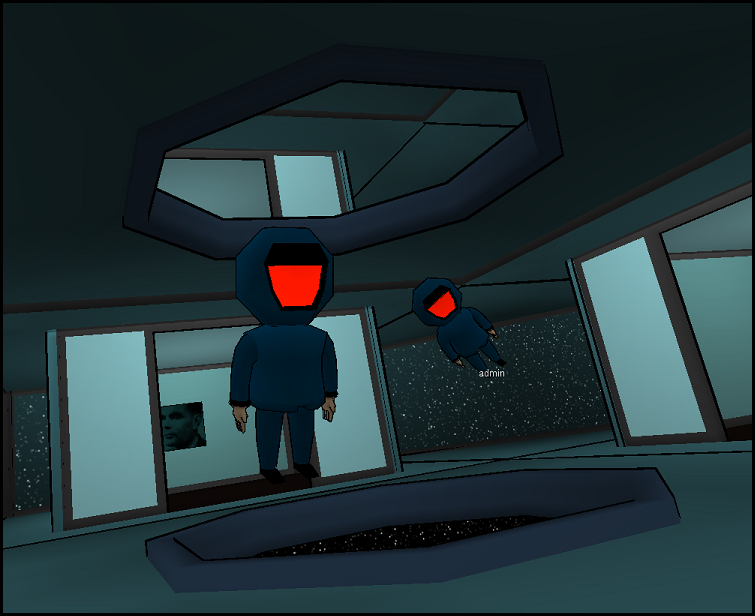
\includegraphics[width=0.30\linewidth]{images/starfall.png}&
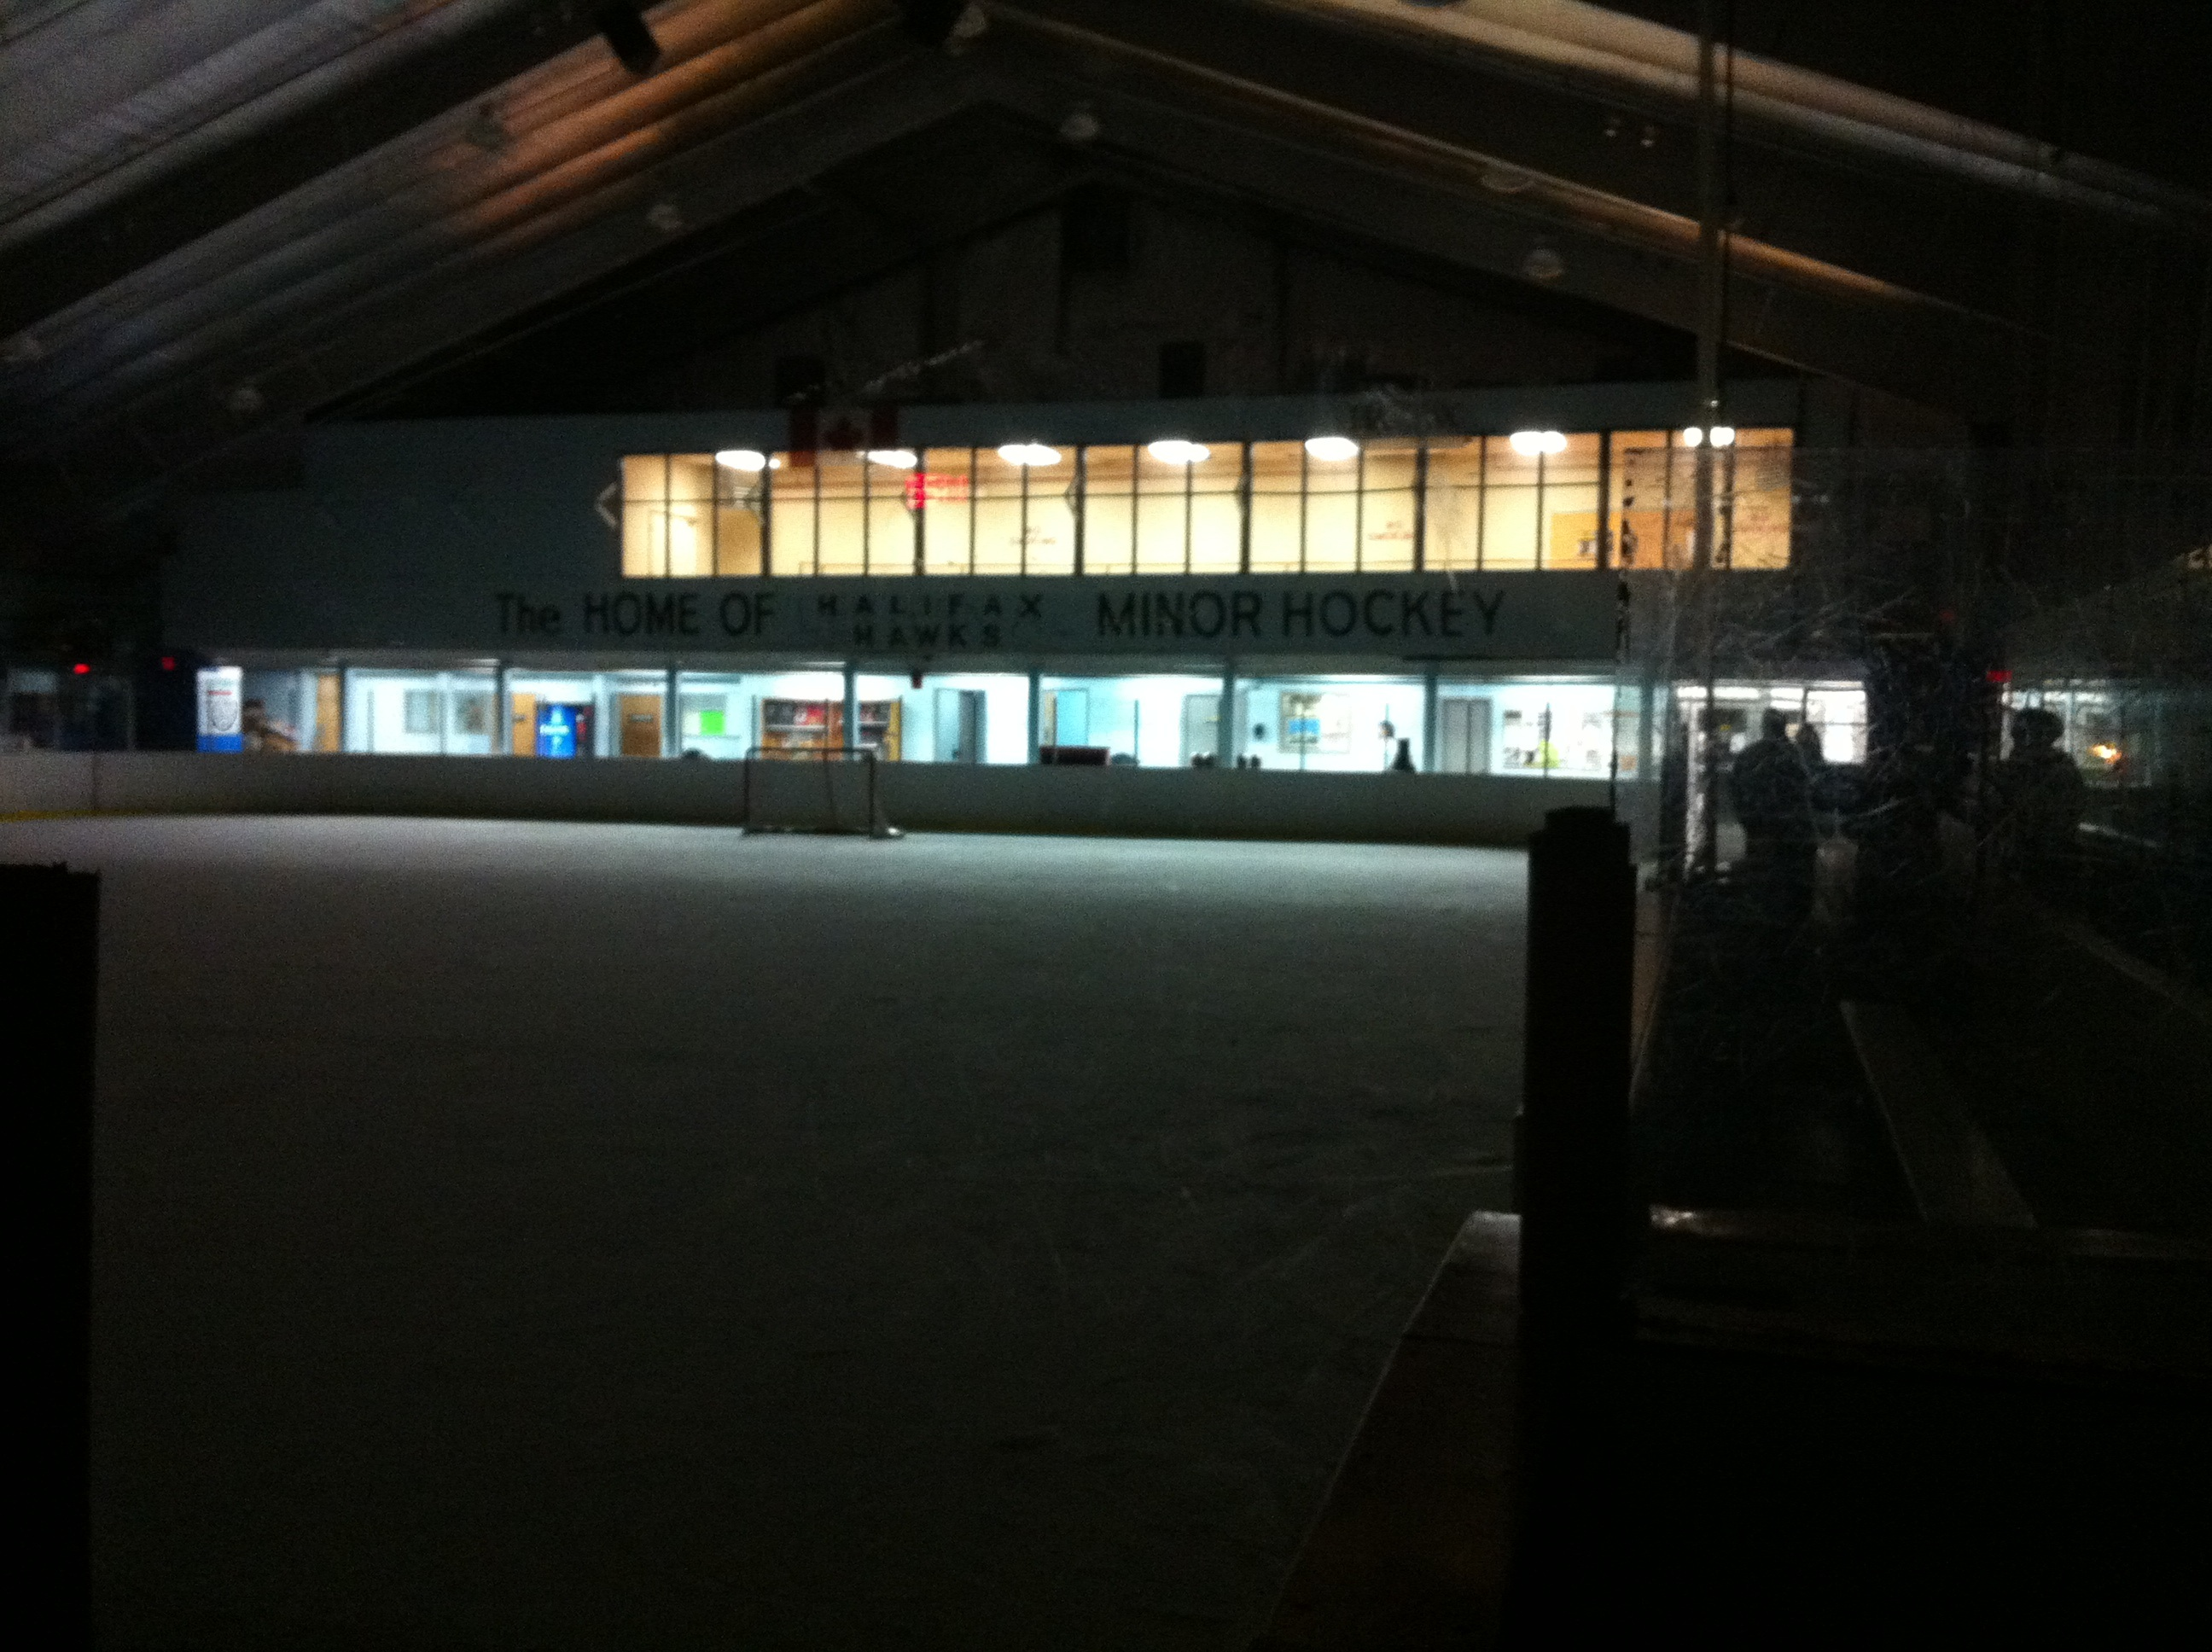
\includegraphics[width=0.30\linewidth]{images/rink.jpg} \\
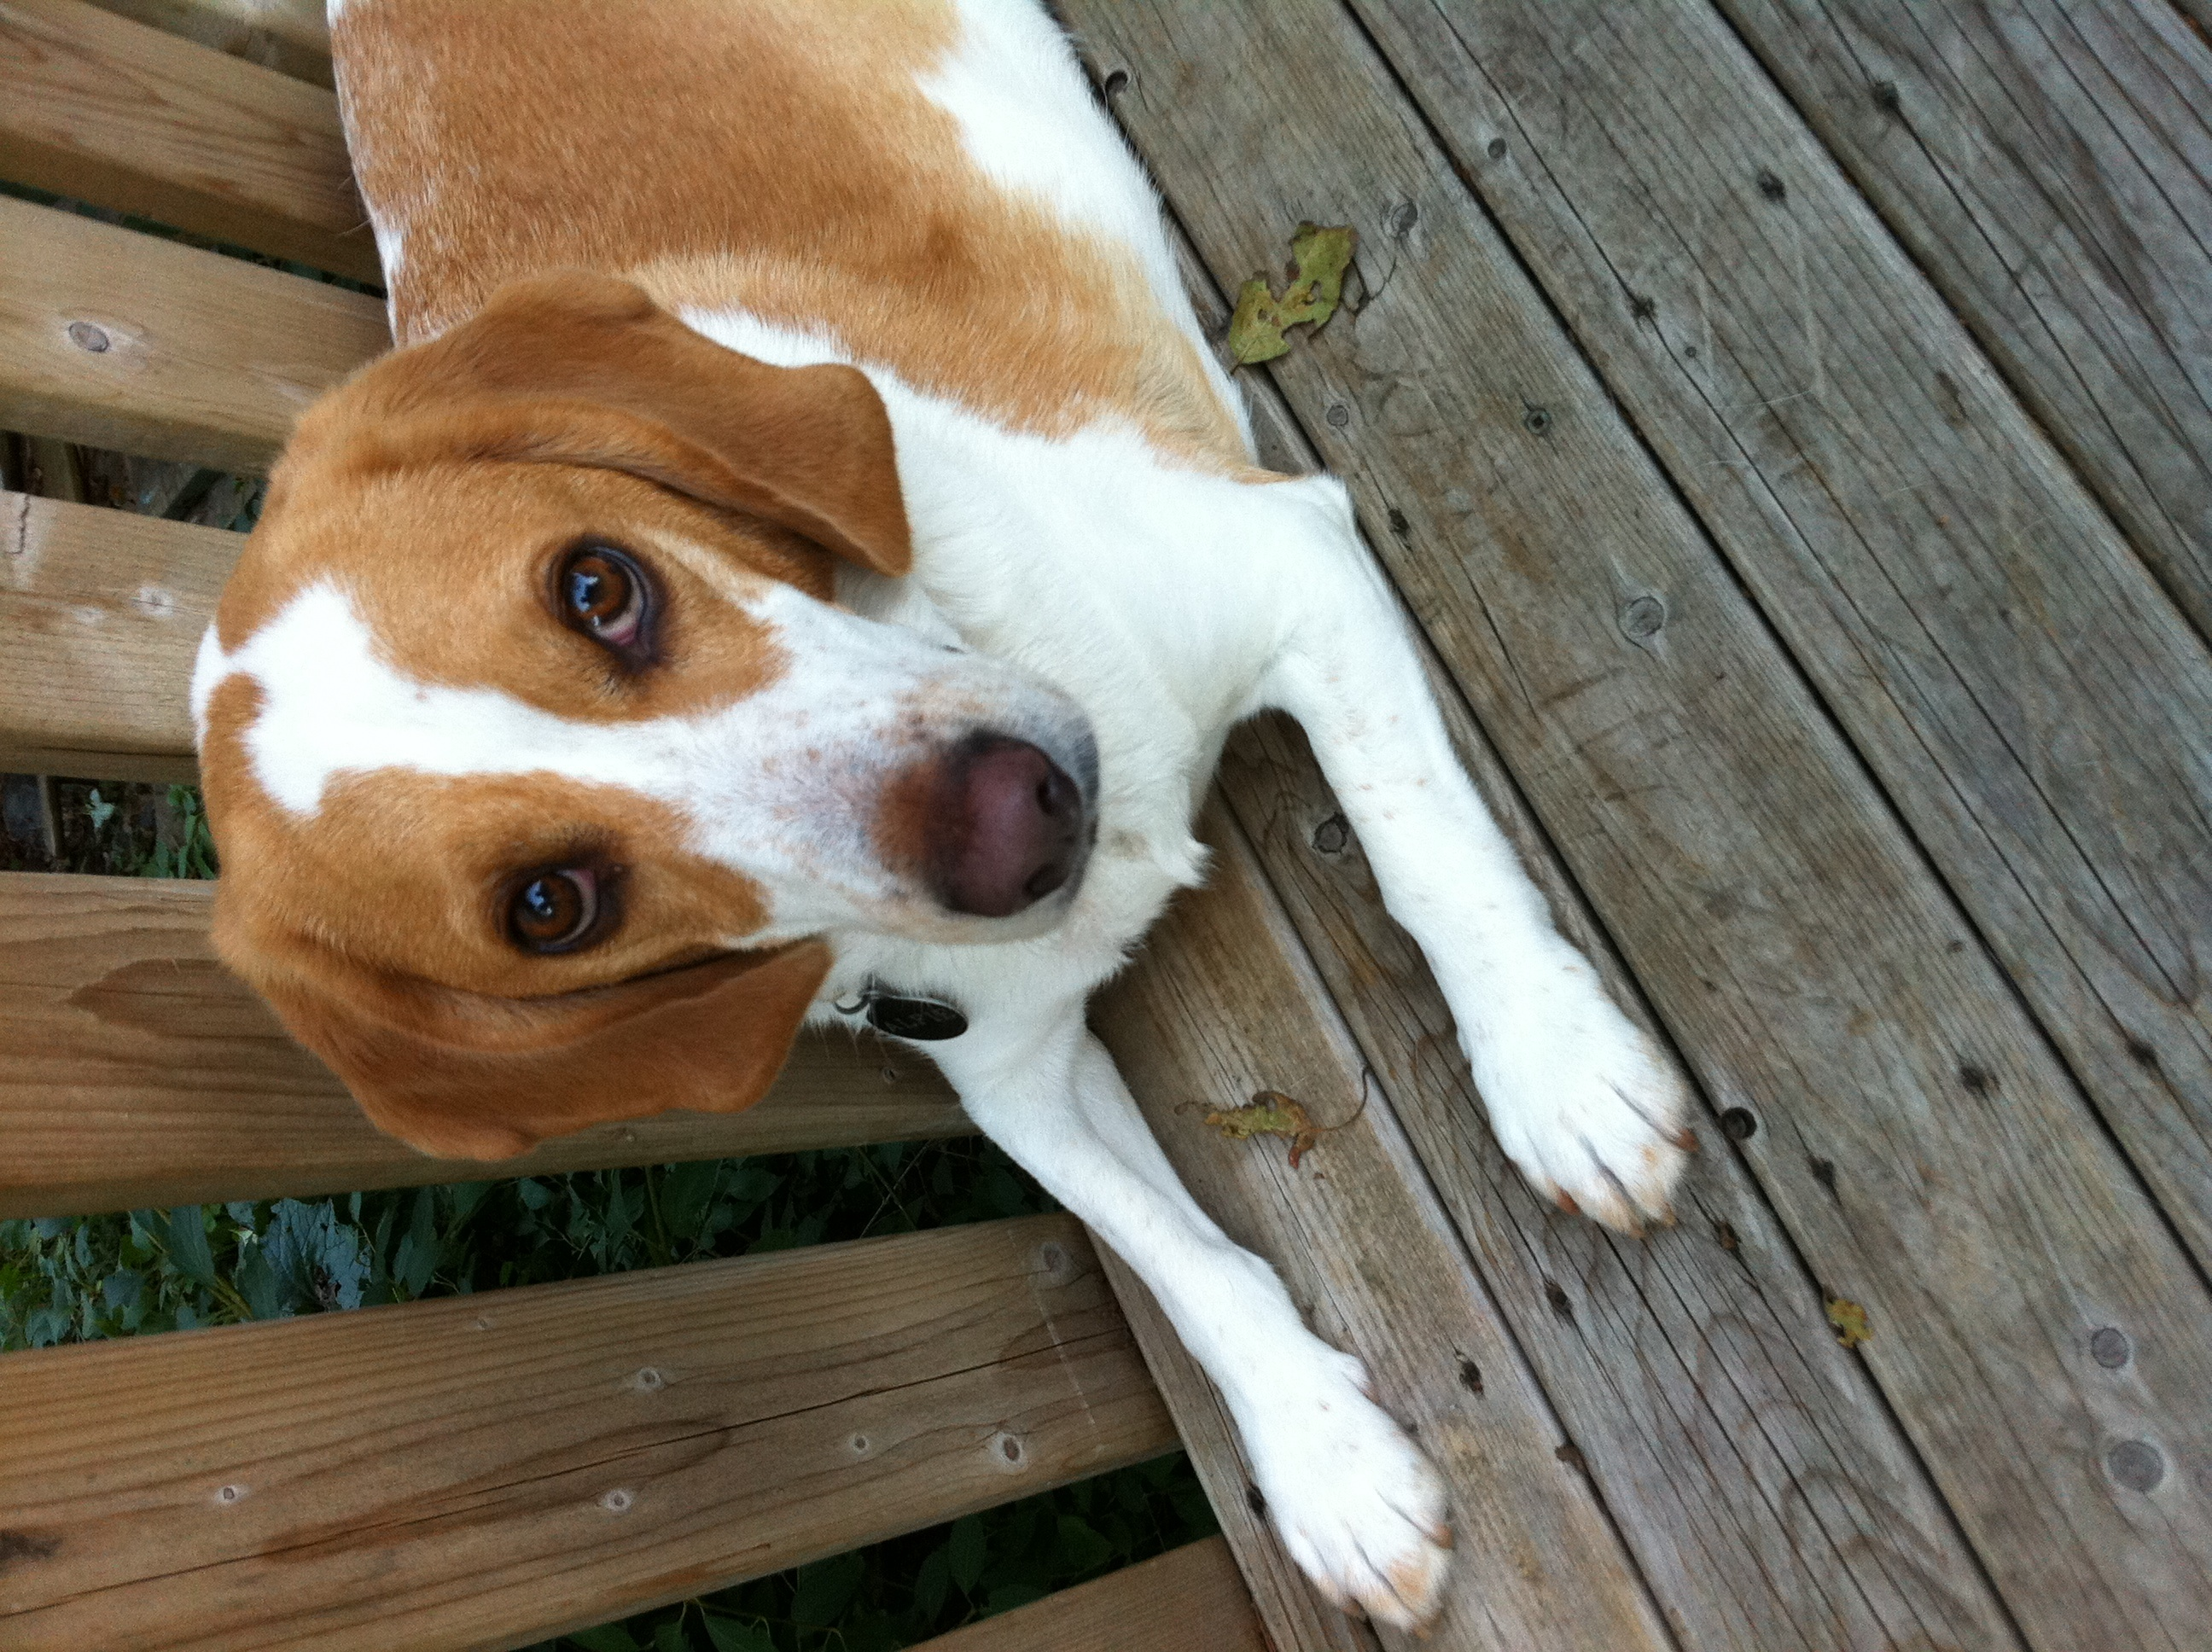
\includegraphics[angle=270, origin=c, width=0.30\linewidth]{images/alfie.jpg}&
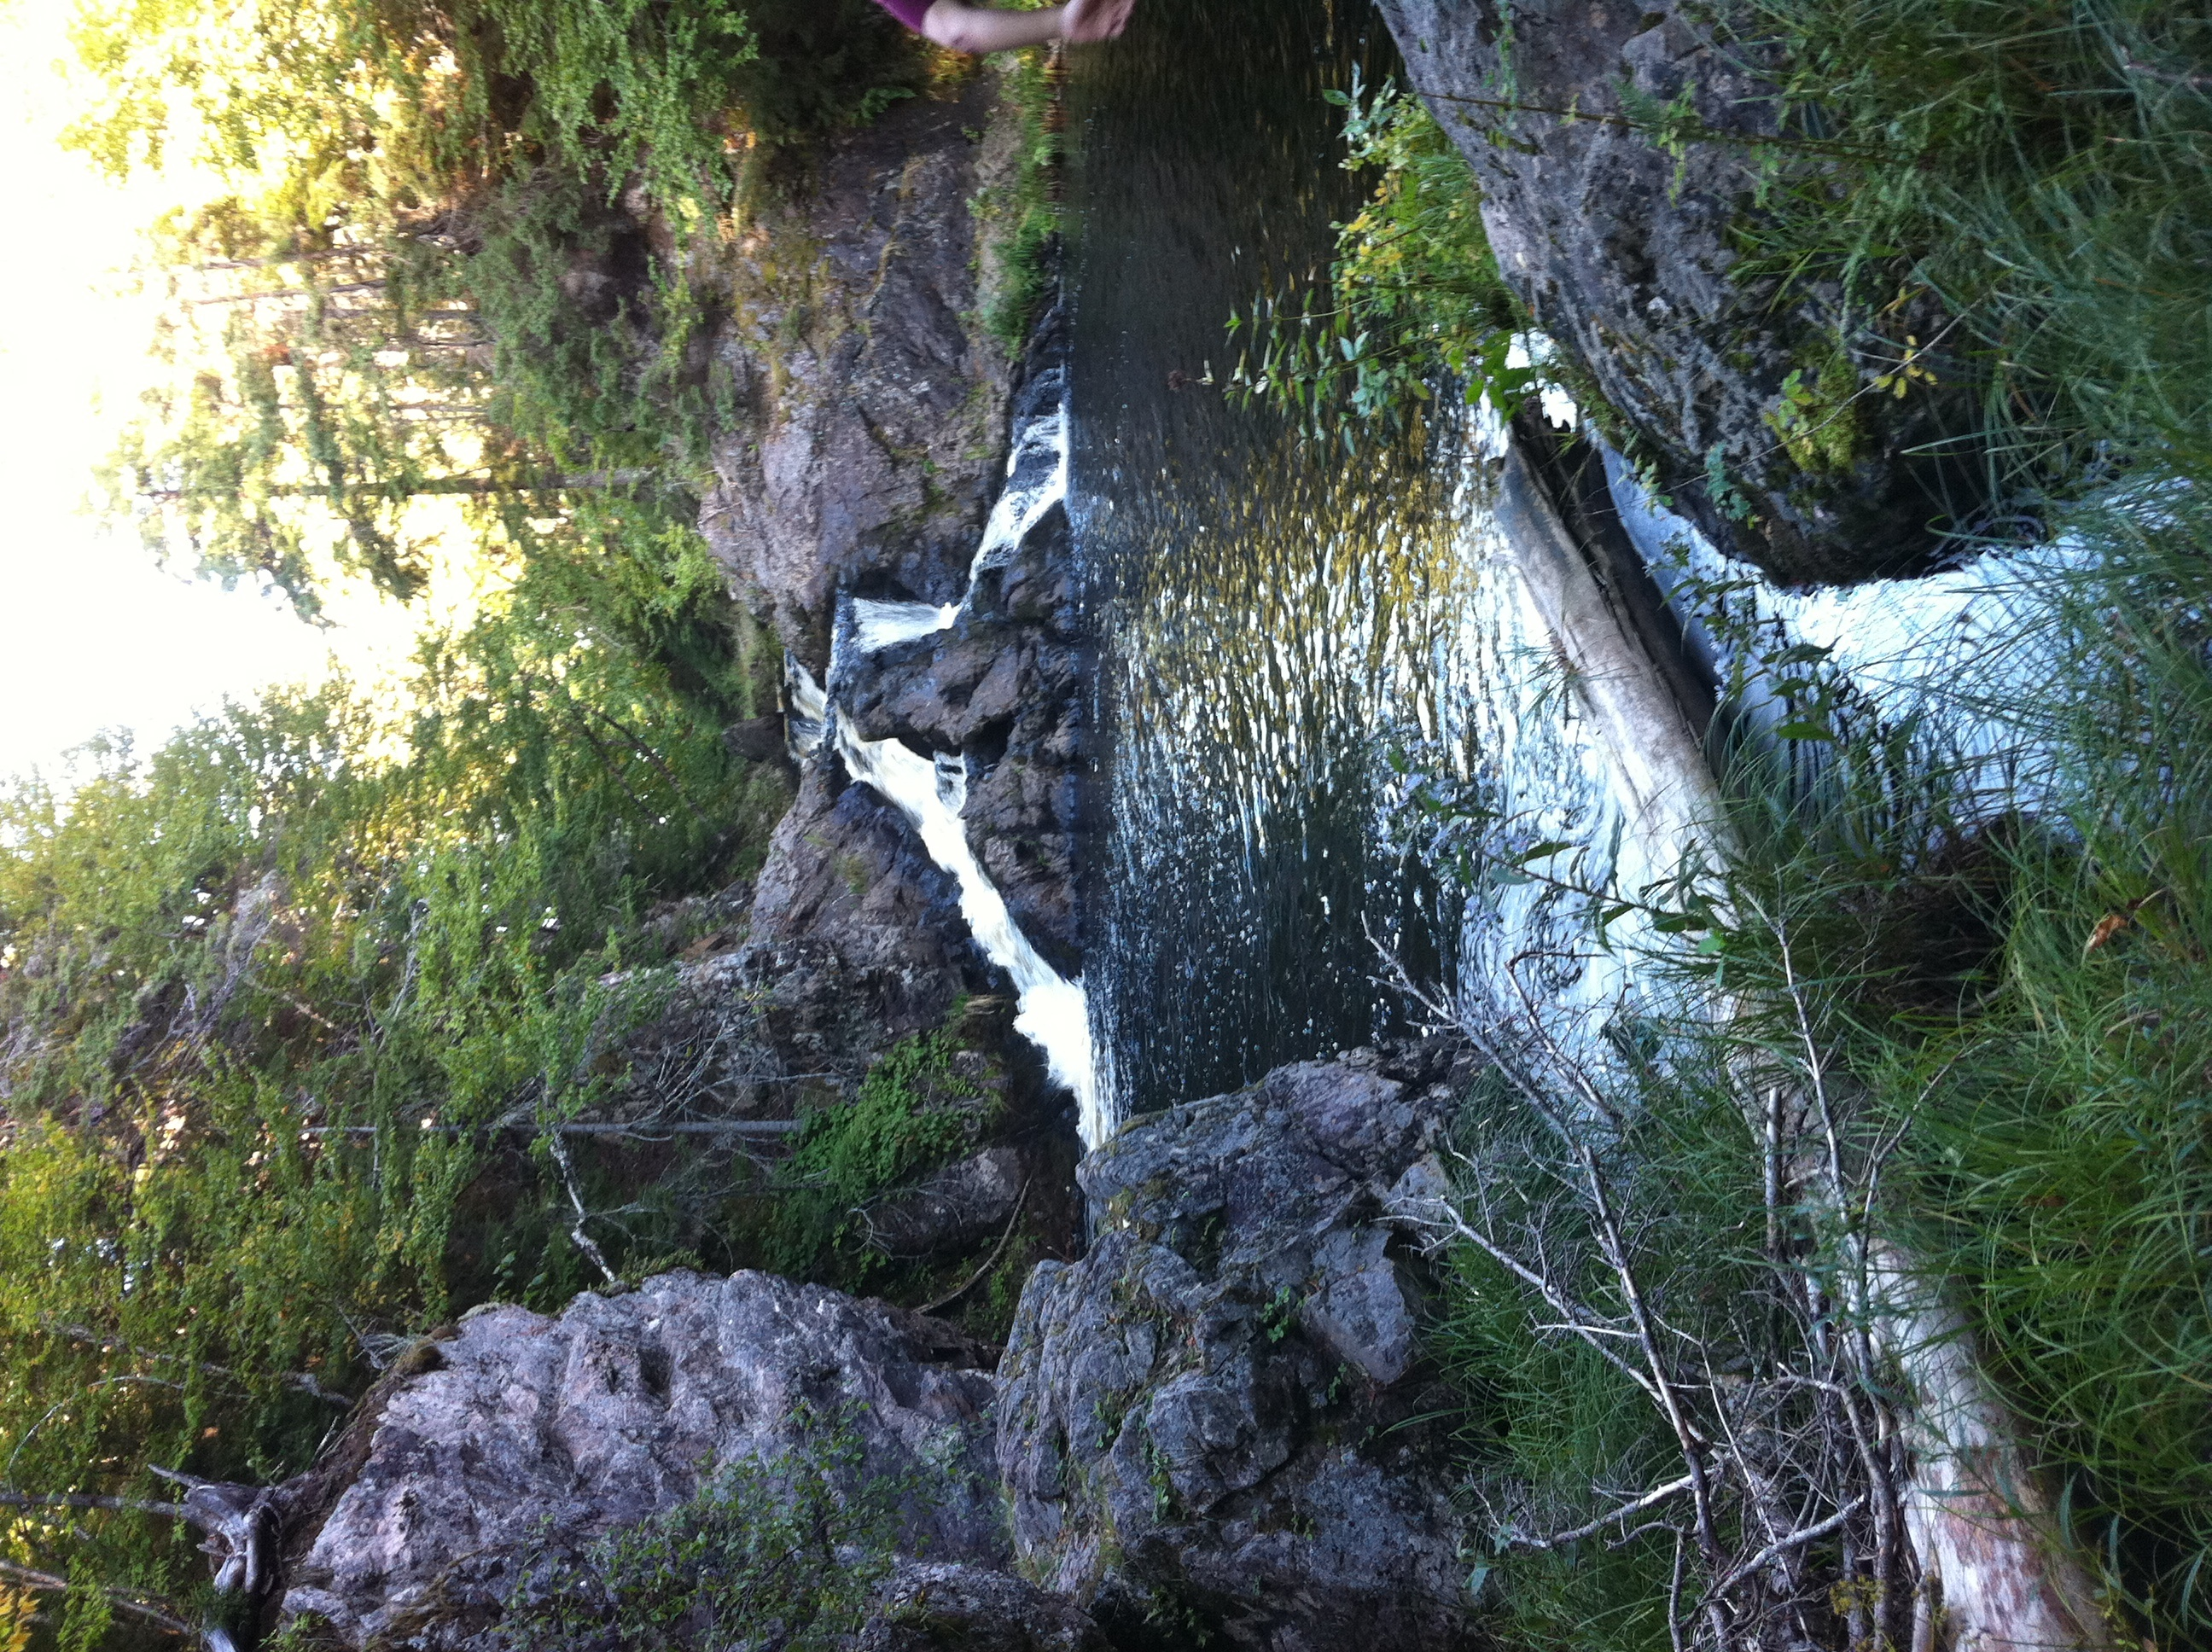
\includegraphics[angle=270, origin=c, width=0.30\linewidth]{images/camping.jpg}\\
\end{tabular}

\end{frame}

\begin{frame}
\frametitle{Where I'm from}
\framesubtitle{Atlantic Canada}
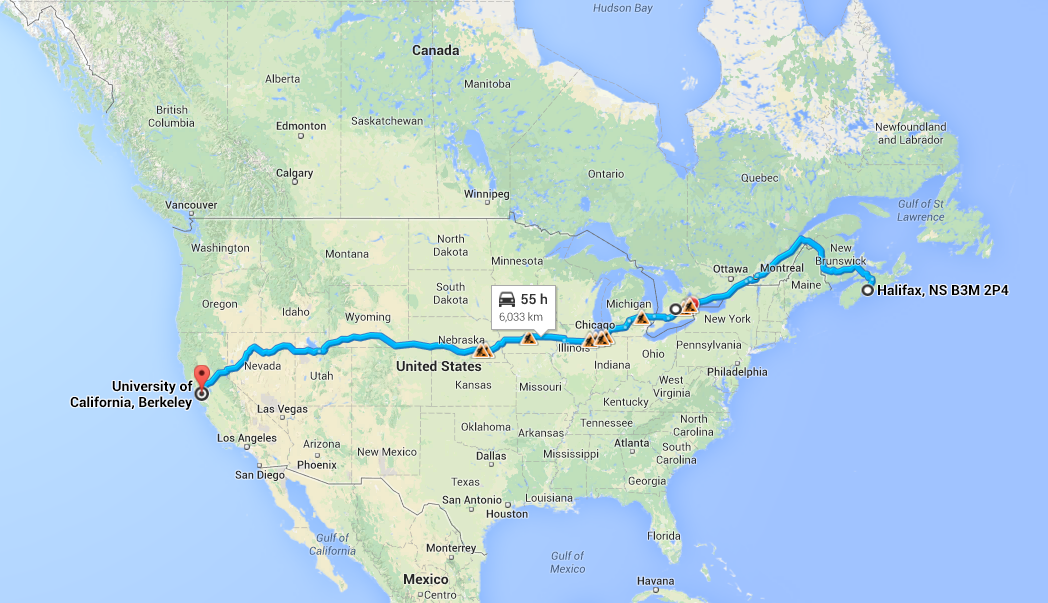
\includegraphics[width=1.0\linewidth]{images/map.png}
\end{frame}

\begin{frame}

\frametitle{What I'm Studying}

\begin{columns}[l]
\begin{column}{.7\textwidth}
\begin{description}
\item[Year] 2
\item[Program] Bachelor of Computer Science
\item[Faculty] Mathematics
\item[Institution] University of Waterloo
\item[Location] Waterloo, Ontario, Canada
\end{description}
\end{column}
\begin{column}{.3\textwidth}
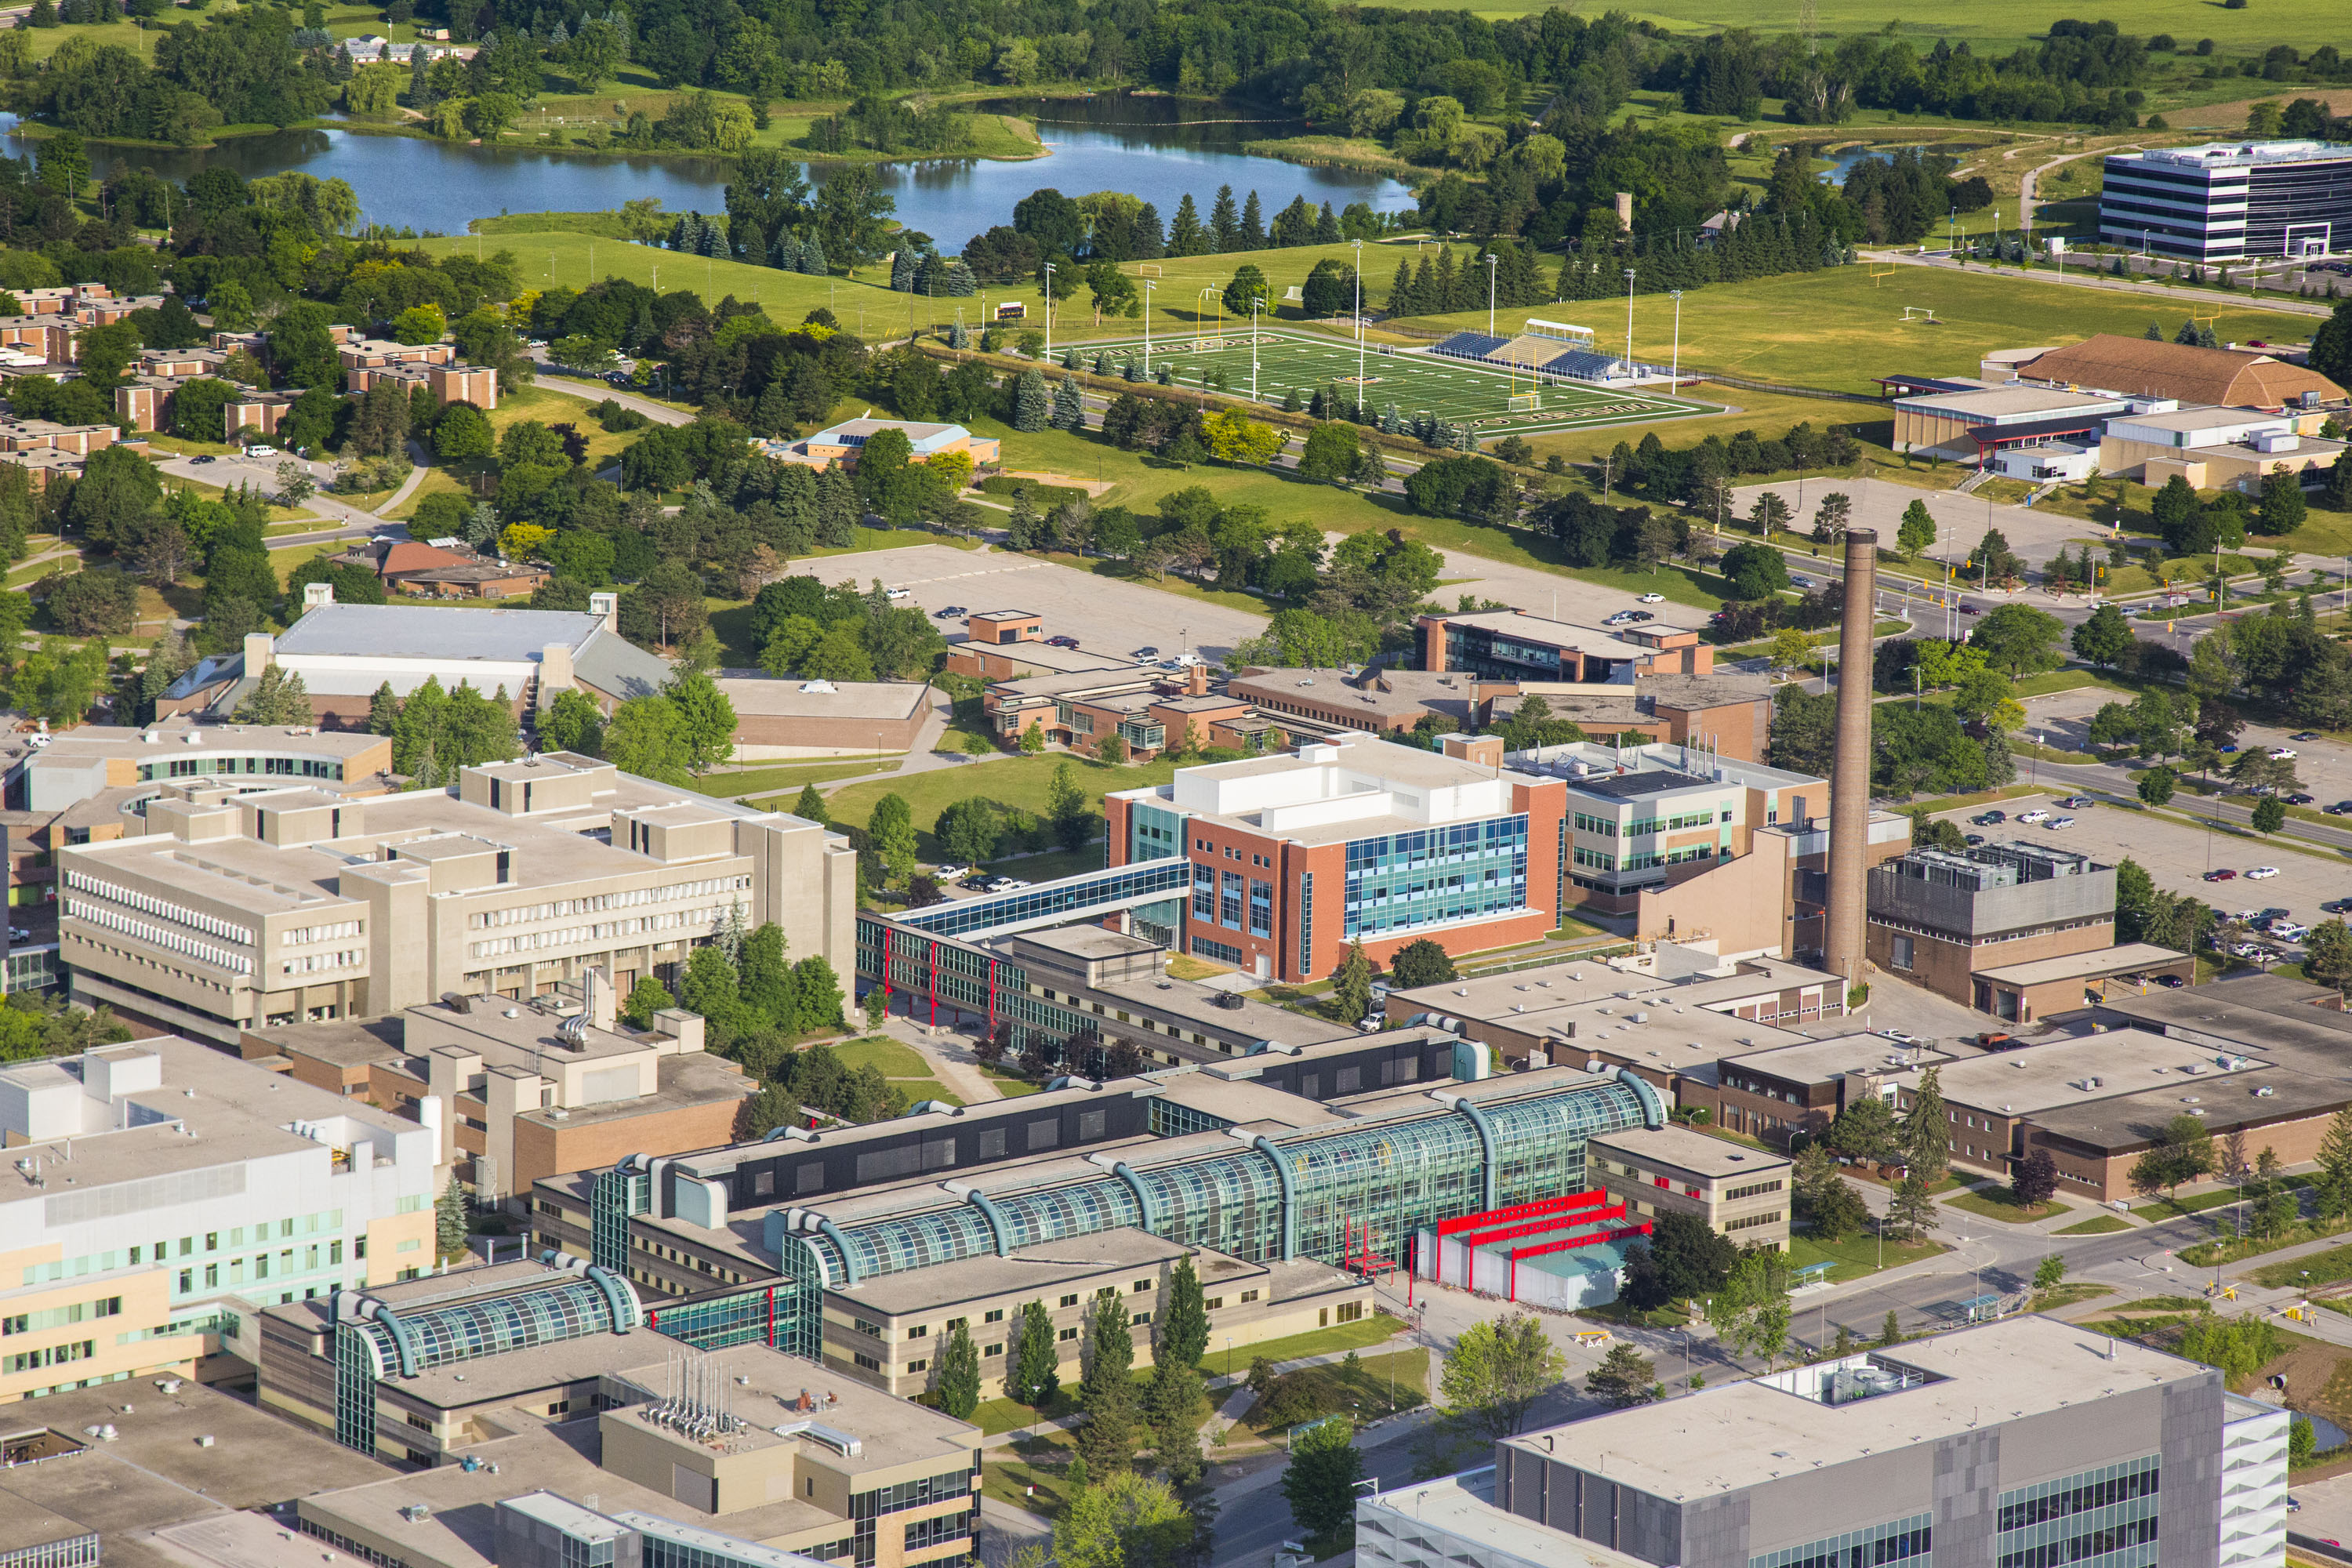
\includegraphics[width=1.0\linewidth]{images/campus.jpg}
\end{column}
\end{columns}

\end{frame}

\begin{frame}

\frametitle{How I Became a Researcher at CREA}
\framesubtitle{Prof. Garan Emailed the University of Waterloo Computer Science Club}

\centering
\begin{tabular}{c c}
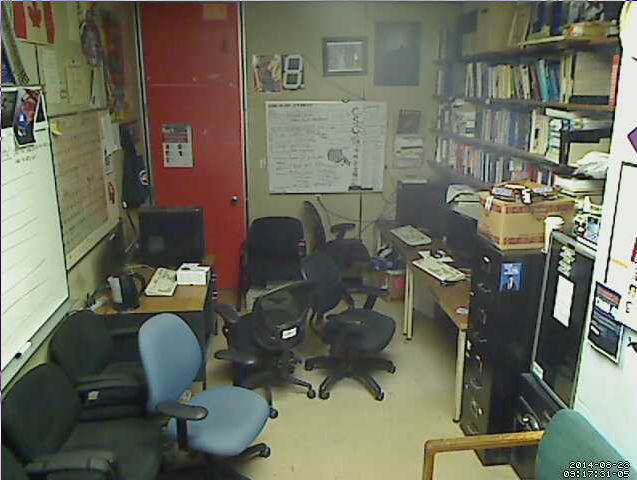
\includegraphics[width=0.40\linewidth]{images/malto_webcam.png} &
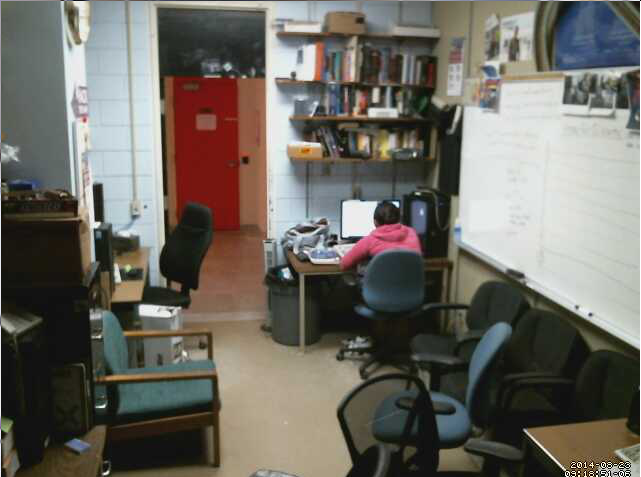
\includegraphics[width=0.40\linewidth]{images/bitshift_webcam.png}\\

\includegraphics[width=0.40\linewidth]{images/csc.png} &
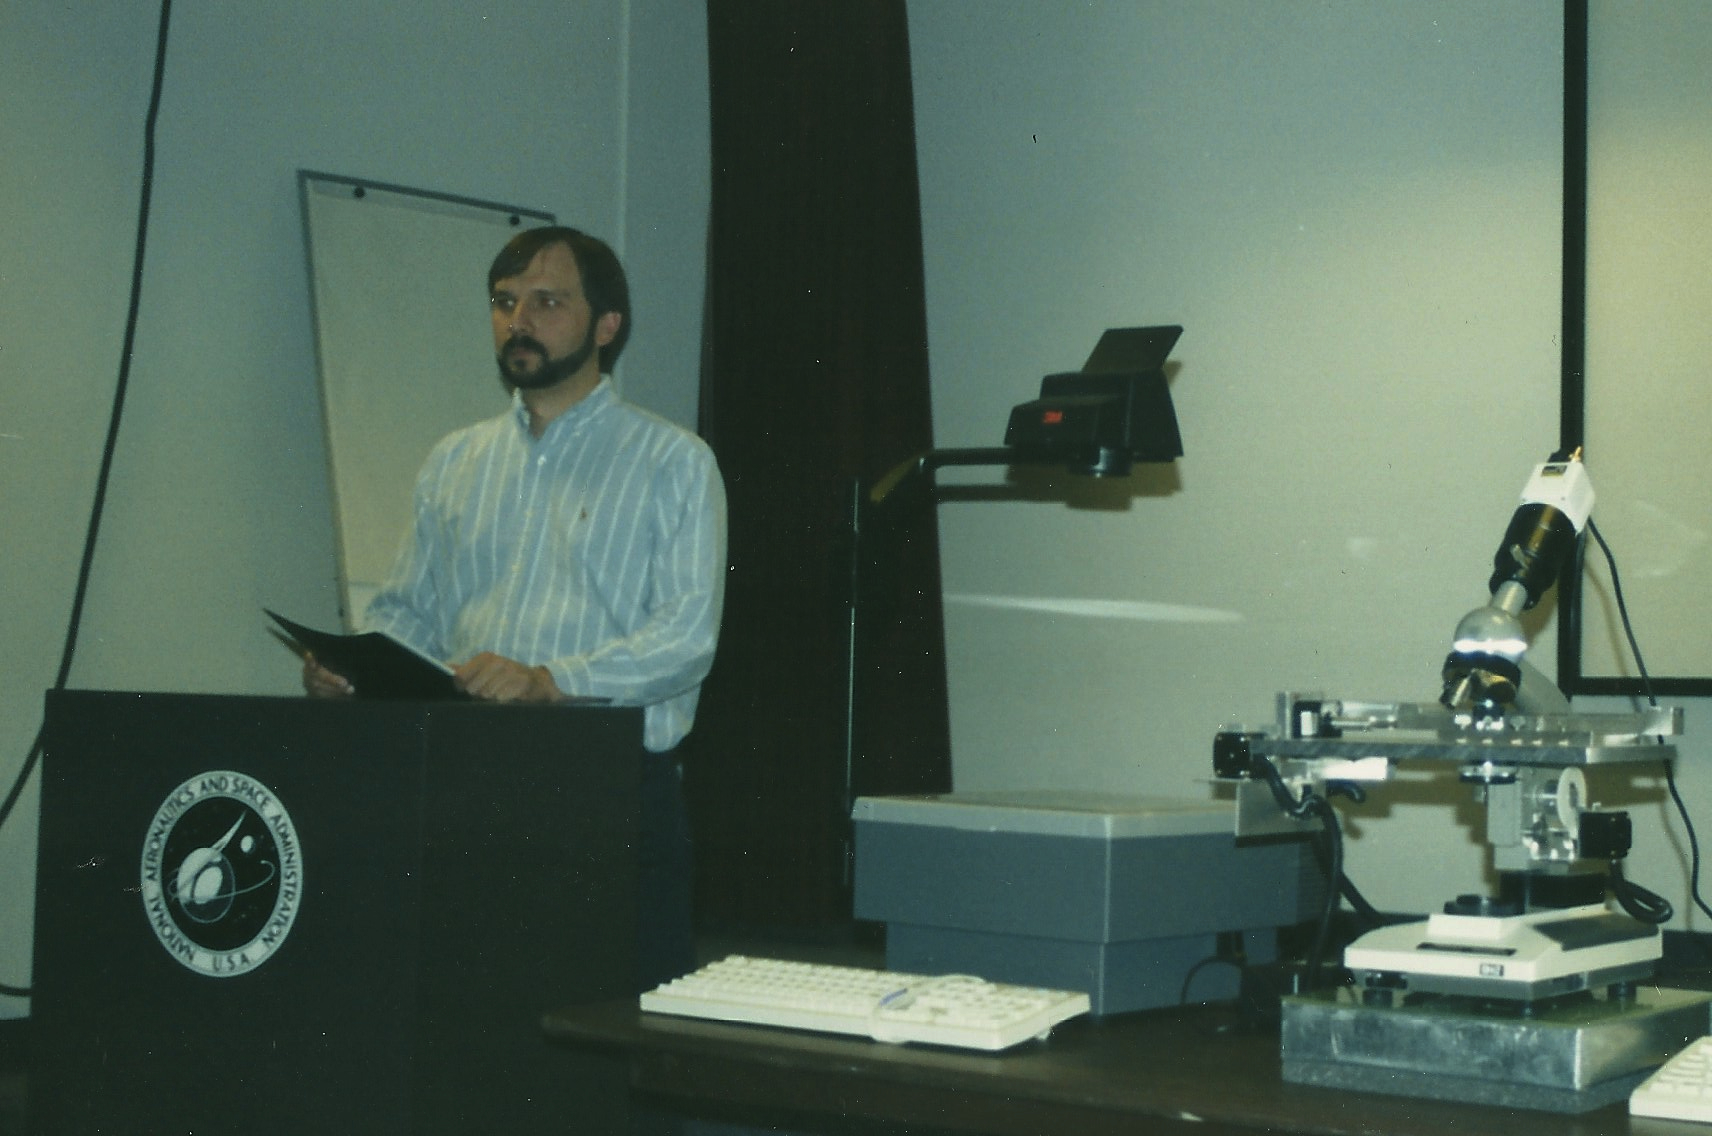
\includegraphics[width=0.40\linewidth]{images/steve_garan.jpg}\\
\end{tabular}

\end{frame}

\begin{frame}

\frametitle{Why was I Interested in Research at CREA?}

\centering
\begin{tabular}{ c | c }
Hobby & CREA Research \\
\hline
Reverse Engineering & Natural Language Processing\\
Game Development & Artificial Intelligence\\
Health & Bioinformatics\\
\end{tabular}

\end{frame}

\section{Automatically Constructing Knowledge Bases}

\begin{frame}

\frametitle{Overview}

\begin{itemize}[<+->]

\item CREA is constructing a knowledge base to study and
understand the human aging process.
\item New discoveries are published quickly and in large
volume.
\item It is infeasible to construct the knowledge base by
hand.
\item Working on software to construct the knowledge base
automatically.

\end{itemize}

\end{frame}

\begin{frame}

\frametitle{Introduction}
\framesubtitle{How to Automatically Construct the Knowledge Base}

\begin{itemize}[<+->]

\item Routinely search for keywords related to aging, dowloading
text articles from sources like PubMed.
\item Build a spam filter to get rid of non-scientific sentences.
\item Extract scientific facts from the sentences and save them
in a structured format.
\item Provide a graphical interface that allows users to search
and otherwise explore the knowledge base.

\end{itemize}

\end{frame}

\section{Extracting Facts in a Structured Format}

\begin{frame}

\frametitle{Information Extraction and Visualization}
\framesubtitle{Overview of Progress}

\centering

\begin{block}{Input}
... The enzymatic cross-links \textcolor{orange}{pyridinoline} and \textcolor{orange}{desmosine} were \textcolor{pink}{examined}
as \textcolor{orange}{candidate sensitizer chromophores} \textcolor{pink}{contained} in \textcolor{orange}{collagen} and \textcolor{orange}{elastin},
respectively. ...
\end{block}

\begin{block}{Output}
\centering
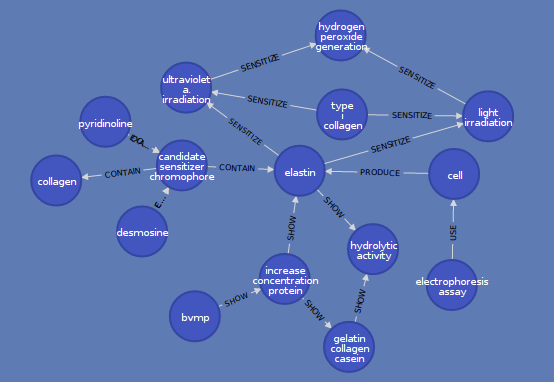
\includegraphics[width=0.5\linewidth]{images/elastinneighborhood.png}
\end{block}

\end{frame}


\begin{frame}

\frametitle{Information Extraction}
\framesubtitle{Method}

\begin{description}[<+->]

\item[Tokenization] Input a text document and read it, one sentence at a time.
\item[Parsing] For each sentence, generate a constituent tree that describes its phrase structure.
\item[Compilation] Extract facts by pattern matching on each constituent tree.

\end{description}

\end{frame}

\begin{frame}

\frametitle{Constituent Tree Tags}
\framesubtitle{Word Level}

\centering

\begin{tabular}{c | c | c}
Tag & Meaning & Example \\
\hline
DT & Determiner & the \\
IN & Preposition & of\\
JJ & Adjective & blue\\
RB & Adverb & quickly\\
CC & Coordinating Conjunction & and \\
NN & Singular Noun & monkey\\
NNS & Plural Noun & monkeys\\
VB & Base Verb & fall\\
VBZ & Singular Present Verb & falls\\
VBD & Past Tense Verb & fell\\
VBN & Past Participle Verb & fallen\\
VBG & Gerund Verb & falling\\
... & ... & ...\\
\end{tabular}

\end{frame}

\begin{frame}

\frametitle{Constituent Tree Tags}
\framesubtitle{Phrase Level}

\centering

\begin{tabular}{c | c | c}
Tag & Meaning & Example \\
\hline
NP & Noun Phrase & the woman \\
VP & Verb Phrase & calls the man \\
PP & Prepositional Phrase & from the store \\
ADVP & Adverb Phrase & quickly and quietly \\
ADJP & Adjective Phrase & blue and red \\
CONJP & Conjunctive Phrase & as well as \\
... & ... & ...\\
\end{tabular}

\end{frame}


\begin{frame}

\frametitle{Constituent Tree Tags}
\framesubtitle{Clause Level}

\centering

\begin{tabular}{c | c | c}
Tag & Meaning & Example \\
\hline
S & Declarative Clause & the dog walks\\
SBAR & Conjunction + Clause & that the dog walks\\
... & ... & ...\\
\end{tabular}

\end{frame}

\begin{frame}

\frametitle{Information Extraction}
\framesubtitle{Example}

\only<1>{
\begin{block}{Input Token}
The man walks the dog.
\end{block}
}

\only<2>{
\begin{block}{Parse Token}
\Tree [.ROOT [.S [.@S [.NP [.DT The ] [.NN man ] ] [.VP [.VBZ walks ] [.NP [.DT the ] [.NN dog ] ] ] ] [.. ] ] ]
\end{block}
}

\only<3>{
\begin{block}{Compile Token}
\Tree [.ROOT [.S [.@S [.NP [.DT The ] [.NN man ] ] [.$\langle$predicate:walk$\rangle$ [.NP [.DT the ] [.NN dog ] ] ] ] [.. ] ] ]
\end{block}
}

\only<4>{
\begin{block}{Compile Token}
\Tree [.ROOT [.$\langle$predicate:walk$\rangle$ [.NP [.DT The ] [.NN man ] ] [.NP [.DT the ] [.NN dog ] ] ] ]
\end{block}
}

\only<5>{
\begin{block}{Compile Token}
\Tree [.ROOT [.$\langle$predicate:walk$\rangle$ $\langle$argument:man$\rangle$ $\langle$argument:dog$\rangle$ ] ]
\end{block}
}

\only<6>{
\begin{block}{Output Fact} walk(man, dog).\end{block}
}

\only<7>{
\begin{block}{Output Fact}
\centering
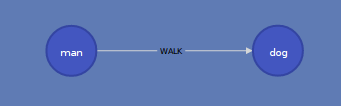
\includegraphics[width=.5\linewidth]{images/manwalkdog.png}
\end{block}
}

\end{frame}

\section{Results \& Discussion}

\begin{frame}

\frametitle{Software Demonstration}
\framesubtitle{A preview of CREA's knowledge base, compiled from
PubMed abstracts.}

\href{http://markfarrell.ca/creal}{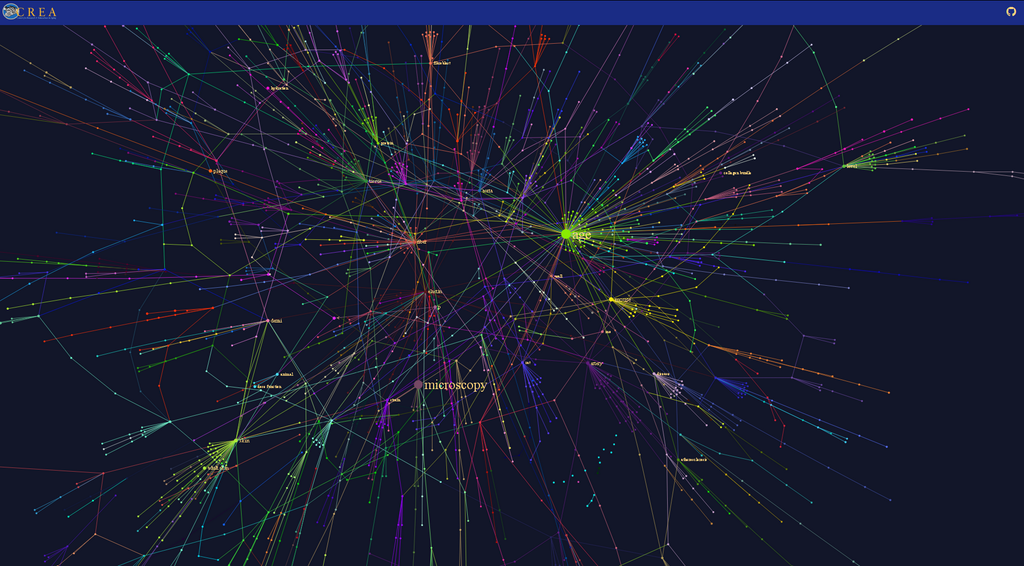
\includegraphics[width=1.0\linewidth]{images/results.png}}

\end{frame}

\begin{frame}

\frametitle{High Performance}
\framesubtitle{Facts can be extracted from many sentences at the same time.}
% It is possible to extract facts from many sentences at the same time.

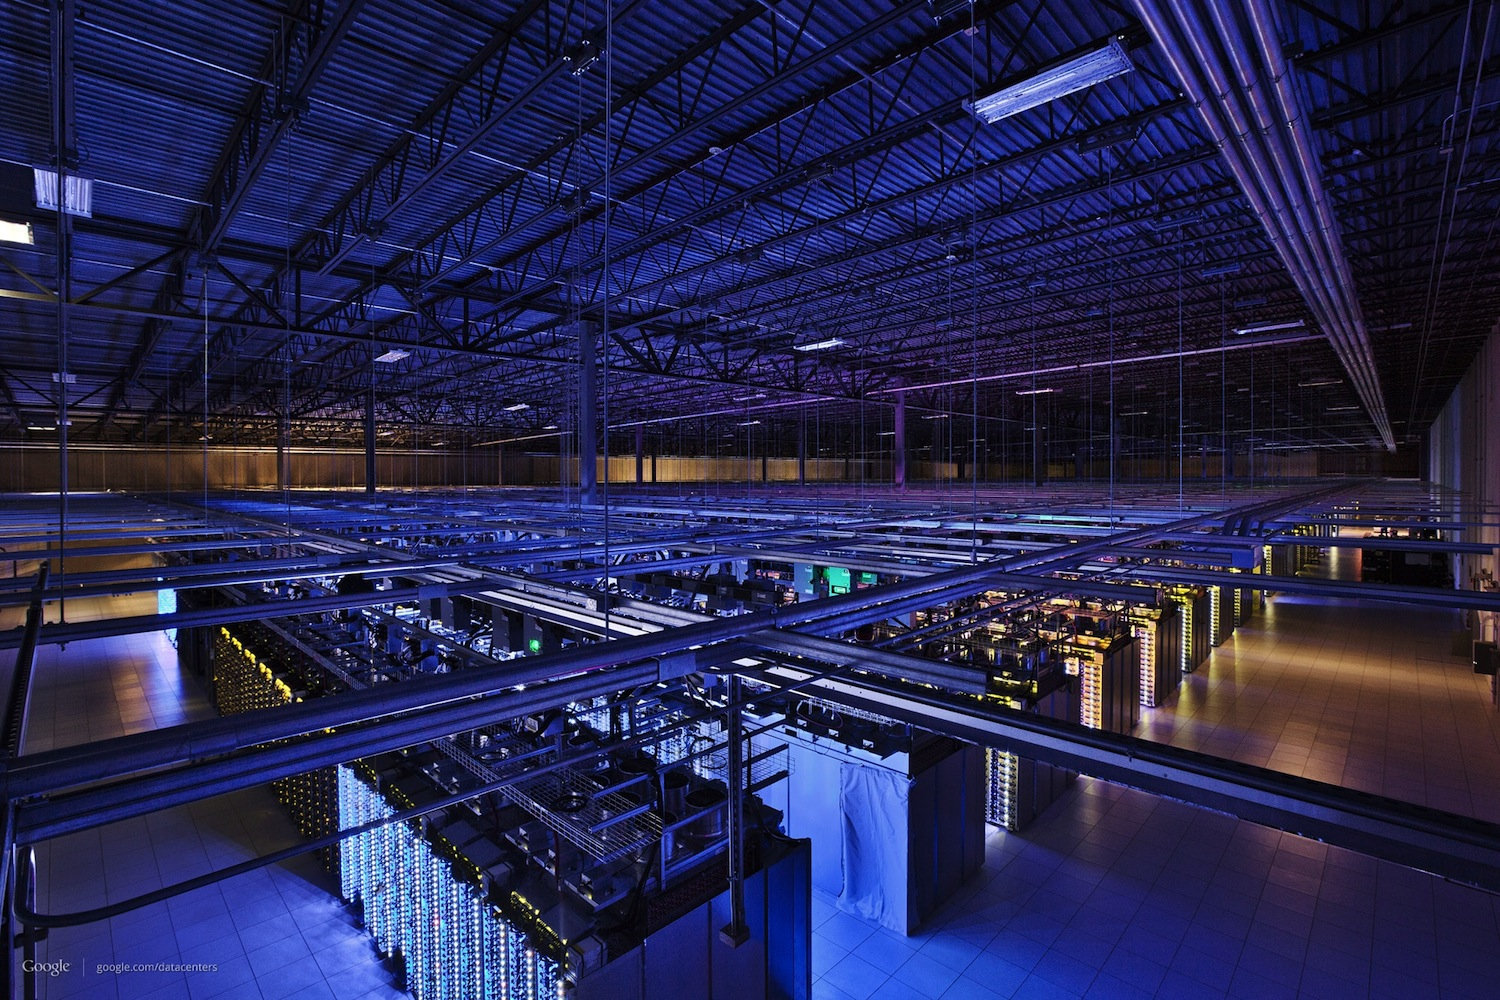
\includegraphics[width=1.0\linewidth]{images/parallel.jpg}

\end{frame}

\begin{frame}

\frametitle{Accuracy}

\begin{itemize}[<+->]

\item Filter spam sentences from documents.

\item The accuracy of the parser could be optimized:
\begin{itemize}[<+->]

\item Should be trained to identify more nouns from the biomedical
domain.

\end{itemize}

\item Define more patterns for extracting facts:
\begin{itemize}[<+->]

\item The software succeeds around 50\% of the time.

\end{itemize}

\end{itemize}

\end{frame}

\begin{frame}

\frametitle{Missing Features}

\begin{itemize}[<+->]

\item Support negated clauses and conditional logic.

\item Facts can contradict each other:
\begin{itemize}[<+->]
\item Store the probability that is true as the weight of its edge on the
knowledge base's graph.
\end{itemize}

\item Scale and launch the software service.

\end{itemize}

\end{frame}

\begin{frame}

\frametitle{Conclusion}

\begin{itemize}[<+->]

\item Demonstrated a method for automatically constructing CREA's
knowledge base on aging.
\item Showed how to extract facts from English text in the knowledge
base's structured format.
\item Discussed the need to improve software accuracy by lensing in on
the biomedical domain.
\item Suggested how the software implementation can be scaled for
production usage.

\end{itemize}

\end{frame}

\end{document}
